\documentclass[letterpaper, 10 pt, conference]{ieeeconf}

\IEEEoverridecommandlockouts
\overrideIEEEmargins

\usepackage{cite}
\usepackage{amsmath,amssymb,amsfonts}
\usepackage{algorithmic}
\usepackage{graphicx}
\usepackage{textcomp}
\usepackage{placeins}

\newtheorem{theorem}{Theorem}[section]
\newtheorem{lemma}[theorem]{Lemma}
\newtheorem{proposition}[theorem]{Proposition}
\newtheorem{corollary}[theorem]{Corollary}
\newtheorem{definition}[theorem]{Definition}
\newtheorem{remark}[theorem]{Remark}
\newtheorem{assumption}[theorem]{Assumption}

\title{\LARGE \bf An Adaptive-Gain Super-Twisting Observer for Sensorless\\ Identification of Differential-Drive Robots}

\author{Laith Alsheikh$^{1}$
\thanks{$^{1}$L. Alsheikh is with the Department of Robotics and Intelligent Systems, Faculty of Engineering, Manara University, Latakia, Syria. \texttt{Laith.Alsheikh@manara.edu.sy}}}

\begin{document}

\maketitle
\thispagestyle{empty}
\pagestyle{empty}

\begin{abstract}
Sensorless identification of the inertial parameters of a differential-drive robot from motor current measurements relies on a super-twisting observer to reconstruct wheel velocity from the back-electromotive-force term. Existing constant-gain realizations require a numerical bound on the wheel angular acceleration, derived from the same mechanical parameters that the identification seeks to estimate, which makes the design circular. This letter removes the requirement through a qualitative boundedness assumption and a boundary-layer adaptive gain law. A self-contained finite-time gain-crossing result shows that the adaptive gain dominates any finite, possibly unknown, disturbance bound, and standard adaptive-gain super-twisting convergence is invoked with its hypotheses verified for the resulting error dynamics. In simulation, the observer generalizes without retuning over a sixfold variation in chassis mass and an eightfold variation in yaw inertia. Among six candidate excitation trajectories, a physically executable alternating drive-and-turn maneuver achieves accuracy comparable to the best, whereas trajectories with markedly lower regressor condition numbers yield worse accuracy, so conditioning and accuracy are governed by distinct mechanisms. A noise-induced bias in the viscous-damping estimate is characterized as a limitation.
\end{abstract}

\section{Introduction}
\label{sec:introduction}
Estimating wheel velocity from motor current, without recourse to encoders or an inertial measurement unit, is an attractive means of identifying the inertial parameters of a mobile robot. The back-electromotive-force term of the armature current equation carries the velocity information, and a finite-time exact differentiator based on the super-twisting algorithm \cite{Levant1998,Moreno2012} can be used to recover it. Existing constant-gain realizations of such observers require the observer gain to dominate a Lipschitz bound on the derivative of the disturbance term, in this case a bound on the wheel angular acceleration, which is fixed a priori from the electrical and mechanical parameters of the plant.

Such a requirement poses no difficulty when the observer is used solely for control purposes. It becomes circular, however, when the observer forms part of a system identification pipeline intended to recover the same mechanical parameters from which its gain is derived, since the gain design would then presuppose knowledge of the very quantities the pipeline is meant to estimate. In the differential-drive setting considered here, the required bound depends on the chassis mass and yaw inertia through the effective-inertia matrix introduced in Section~\ref{sec:model}, which are precisely the parameters identified in Section~\ref{sec:rls}.

\emph{Contribution.} The contribution of this letter is to replace the numerical acceleration bound with a qualitative boundedness assumption and a boundary-layer adaptive gain law (Section~\ref{sec:observer}), following the methodology of \cite{Plestan2010,Shtessel2012} and adapted here to a current-based velocity observer in the manner of \cite{Bahrami2020}. A self-contained finite-time gain-crossing result is established (Proposition~\ref{prop:crossing}), showing that the adaptive gain dominates any finite, possibly unknown, disturbance bound in finite time. The standard adaptive-gain super-twisting convergence result is then invoked, with its hypotheses verified for the resulting error dynamics (Theorem~\ref{thm:convergence}), and the design is validated in closed loop. The proposed observer is shown to generalize without retuning across a wide range of unknown plants (Section~\ref{sec:genexp}), and among several candidate excitation trajectories, one is identified that combines high identification accuracy with physical executability on the robot itself (Section~\ref{sec:trajexp}). A noise-induced limitation of the approach is characterized rather than omitted (Section~\ref{sec:discussion}).

\section{System Model}
\label{sec:model}
We consider a differential-drive robot actuated by two independent brushed DC motors (right and left, indexed by $k\in\{R,L\}$) driving wheels of radius $r$ through a fixed gear ratio, with track width $d$. The electrical dynamics of each motor are given by
\begin{equation}
L_a\dot\imath_k = -R_ai_k-K_b\omega_k+u_k, \qquad k\in\{R,L\},
\label{eq:elec}
\end{equation}
with armature current $i_k$, applied voltage $u_k$, and wheel angular velocity $\omega_k$. In isolation, each wheel satisfies the torque balance $J_w\dot\omega_k=K_ti_k-b\omega_k-\tau_{L,k}$, where $\tau_{L,k}$ denotes an unmodeled load-torque disturbance. The rigid-body constraint imposed by the chassis couples the two wheels, so that, expressed in terms of the actual wheel accelerations $(\dot\omega_R,\dot\omega_L)$, the isolated wheel inertia $J_w$ is replaced by an effective inertia that also accounts for a share of the chassis translational and rotational inertia. Eliminating the chassis linear and angular velocities yields
\begin{equation}
\mathbf{M}\begin{bmatrix}\dot\omega_R\\\dot\omega_L\end{bmatrix}+b\begin{bmatrix}\omega_R\\\omega_L\end{bmatrix}=K_t\begin{bmatrix}i_R\\i_L\end{bmatrix}-\begin{bmatrix}\tau_{L,R}\\\tau_{L,L}\end{bmatrix},
\label{eq:mech}
\end{equation}
\begin{equation}
\mathbf{M}=\begin{bmatrix}\alpha&\beta\\\beta&\alpha\end{bmatrix}, \quad
\alpha=J_w+\frac{mr^2}{4}+\frac{I_zr^2}{4d^2},
\label{eq:Mmatrix}
\end{equation}
\begin{equation}
\beta=\frac{r^2(d^2m-I_z)}{4d^2},
\label{eq:beta}
\end{equation}
where $m$ denotes the chassis mass and $I_z$ its yaw moment of inertia.

\emph{Sensing and prior knowledge.} The currents $i_R,i_L$ and applied voltages $u_R,u_L$ are measured, whereas the wheel velocities $\omega_R,\omega_L$ are not, so that the identification pipeline is sensorless with respect to velocity. The electrical parameters $R_a,L_a,K_b,K_t,b$ are assumed known from an independent per-motor bench characterization (locked-rotor and no-load tests) carried out prior to chassis assembly and hence decoupled from the chassis dynamics. The parameters $m$, $I_z$, and $J_w$, and consequently $\alpha$ and $\beta$ in \eqref{eq:Mmatrix}--\eqref{eq:beta}, are not known a priori; their identification, together with that of $b$, from $(i_R,i_L,u_R,u_L)$ alone is the objective of the pipeline described in Section~\ref{sec:rls}. Section~\ref{sec:observer} constructs, for each channel, a velocity estimate $\hat\omega_k$ from \eqref{eq:elec} that requires neither $\alpha,\beta$ nor a bound on $\tau_{L,k}$.

\section{Adaptive-Gain Super-Twisting Observer}
\label{sec:observer}

The electrical dynamics of each channel are given by \eqref{eq:elec}, with $i_k,u_k$ measured and $\omega_k$ unmeasured. Reconstructing $\omega_k$ from $(i_k,u_k)$ by means of a super-twisting observer requires a bound on the derivative of the back-EMF term $\varphi_k(t):=-(K_b/L_a)\omega_k(t)$, or equivalently on $\dot\omega_k$. In a constant-gain design, this bound is derived from the mechanical parameters of the plant, which are precisely the quantities the identification stage of the pipeline is intended to estimate. This requirement is removed in what follows.

\begin{assumption}
\label{as:bounded}
For $k\in\{R,L\}$, $|\dot\omega_k(t)|\le\Delta_k<\infty$ for all $t\ge0$, where $\Delta_k$ need not be known to the designer; only its existence is used. Equivalently, $|\dot\varphi_k(t)|\le\Lambda_k:=(K_b/L_a)\Delta_k<\infty$ with $\Lambda_k$ unknown.
\end{assumption}

\subsection{Observer and error dynamics}
With $e_k:=i_k-\hat\imath_k$, define
\begin{align}
\dot{\hat\imath}_k &= -\frac{R_a}{L_a}\hat\imath_k+\frac{u_k}{L_a}+z_k+\kappa_{1,k}(t)\sqrt{|e_k|}\,\mathrm{sign}(e_k), \label{eq:obs1}\\
\dot z_k &= \kappa_{2,k}(t)\,\mathrm{sign}(e_k), \qquad \hat\omega_k := -\frac{L_a}{K_b} z_k, \label{eq:obs2}
\end{align}
identical in structure to a fixed-gain super-twisting observer, with the difference that $\kappa_{1,k}(t)$ and $\kappa_{2,k}(t)$ are time-varying and governed by the adaptive law of Section~\ref{sec:adaptlaw} rather than computed from a numerical bound. Subtracting \eqref{eq:elec} from \eqref{eq:obs1} and defining $\zeta_k:=\varphi_k(t)-z_k$ yields
\begin{align}
\dot e_k &= -\kappa_{1,k}(t)\sqrt{|e_k|}\,\mathrm{sign}(e_k)+\zeta_k, \label{eq:err1}\\
\dot\zeta_k &= -\kappa_{2,k}(t)\,\mathrm{sign}(e_k)+\dot\varphi_k(t), \qquad |\dot\varphi_k(t)|\le\Lambda_k. \label{eq:err2}
\end{align}

\subsection{Adaptive gain law}
\label{sec:adaptlaw}
Omitting the channel subscript $k$ for brevity, let
\begin{equation}
\dot\kappa_1(t)=
\begin{cases}
\gamma, & |e(t)|>\varepsilon,\\
-\gamma, & |e(t)|\le\varepsilon \text{ and } \kappa_1(t)>\kappa_1^{\min},\\
\gamma, & |e(t)|\le\varepsilon \text{ and } \kappa_1(t)\le\kappa_1^{\min},
\end{cases}
\label{eq:adaptlaw}
\end{equation}
\begin{equation}
\kappa_2(t)=\rho\,\kappa_1(t), \qquad \kappa_1(0)>\kappa_1^{\min}>0,
\label{eq:ratio}
\end{equation}
with $\gamma,\rho,\varepsilon,\kappa_1^{\min}>0$ design constants determined by the observer's own operating characteristics rather than by the plant: $\varepsilon$ is set by the current-sensor noise floor (e.g., $\varepsilon\approx3\sigma_i$), $\gamma$ governs the reaching time, $\rho$ is a free positive ratio, and $\kappa_1^{\min}$ is a small floor value. This boundary-layer switching law follows \cite{Plestan2010,Shtessel2012}.

\subsection{Theoretical guarantees}
\begin{proposition}[Gain crossing]
\label{prop:crossing}
Fix $\rho>0$. If $\kappa_1\ge\kappa_1^\dagger:=\max(2\Lambda/\rho,\,6\rho)$, then $(\kappa_1,\kappa_2{=}\rho\kappa_1)$ satisfies the classical super-twisting sufficient condition \cite{Moreno2012}
\begin{equation}
\kappa_2>\Lambda, \qquad \kappa_1^2 \ge \frac{4\Lambda(\kappa_2+\Lambda)}{\kappa_2-\Lambda},
\label{eq:MO}
\end{equation}
and continues to satisfy it for every $\kappa_1'\ge\kappa_1$. Since $\Lambda$ is finite by Assumption~\ref{as:bounded} and $\kappa_1(t)$ increases at fixed rate $\gamma$ whenever $|e(t)|>\varepsilon$, there is a finite time $T^\ast\le(\kappa_1^\dagger-\kappa_1(0))/\gamma$ by which \eqref{eq:MO} holds, for any finite $\Lambda$, known or not.
\end{proposition}
\begin{proof}
At $\kappa_1=\kappa_1^\dagger$: $\kappa_2-\Lambda=\rho\kappa_1-\Lambda\ge\rho(2\Lambda/\rho)-\Lambda=\Lambda>0$, so the first inequality in \eqref{eq:MO} holds strictly. Since $\Lambda\le\rho\kappa_1/2$, $\kappa_2+\Lambda=\rho\kappa_1+\Lambda\le1.5\rho\kappa_1$, hence
$4\Lambda(\kappa_2+\Lambda)/(\kappa_2-\Lambda)\le4\Lambda(1.5\rho\kappa_1)/\Lambda=6\rho\kappa_1\le\kappa_1^2$
whenever $\kappa_1\ge6\rho$. Both bounds hold simultaneously once $\kappa_1\ge\max(2\Lambda/\rho,6\rho)$, and continue to hold for all larger $\kappa_1$ since the left side of the second inequality grows unboundedly while the right side approaches the finite limit $4\Lambda$.
\end{proof}

\begin{theorem}[Convergence]
\label{thm:convergence}
Under Assumption~\ref{as:bounded}, the observer \eqref{eq:obs1}--\eqref{eq:obs2} with adaptive law \eqref{eq:adaptlaw}--\eqref{eq:ratio} drives $(e_k,\zeta_k)$ into, and thereafter keeps it within, an $O(\varepsilon_k)$ neighborhood of the origin in finite time; consequently $\hat\omega_k\to\omega_k$ up to $O(\varepsilon_k)$.
\end{theorem}
This result is the standard adaptive-gain super-twisting convergence property established in \cite{Plestan2010,Shtessel2012}, applied here to a current-based velocity observer following \cite{Bahrami2020}. Proposition~\ref{prop:crossing} independently verifies its key hypothesis for the error dynamics \eqref{eq:err1}--\eqref{eq:err2}: namely, that a sufficient constant gain pair is reached within finite time.

\begin{proposition}[Bounded gains]
\label{prop:bounded}
$\kappa_{1,k}(t)$ is bounded for all $t\ge0$.
\end{proposition}
\begin{proof}
Suppose, for contradiction, $\kappa_{1,k}(t)\to\infty$. By \eqref{eq:adaptlaw}, $\kappa_{1,k}$ increases only while $|e_k(t)|>\varepsilon_k$, so unbounded growth requires $|e_k(t)|>\varepsilon_k$ for arbitrarily large $t$. But once $\kappa_{1,k}$ exceeds $\kappa_1^\dagger$ (Proposition~\ref{prop:crossing}), Theorem~\ref{thm:convergence} guarantees that $(e_k,\zeta_k)$ enters the $O(\varepsilon_k)$ neighborhood of the origin, and in particular satisfies $|e_k|\le\varepsilon_k$, in finite time; this contradicts $|e_k(t)|>\varepsilon_k$ holding for arbitrarily large $t$. Hence $\kappa_{1,k}(t)$ is bounded.
\end{proof}

\begin{remark}
Neither $R_a,L_a,K_b$, which enter only the observer equation \eqref{eq:obs1} itself and are known from the bench characterization of Section~\ref{sec:model}, nor the mechanical parameters comprising the effective inertia, nor any bound on the disturbance torque, appear in the adaptive law \eqref{eq:adaptlaw}--\eqref{eq:ratio}. The construction relies solely on the qualitative Assumption~\ref{as:bounded}, thereby removing the circularity of requiring the identification target as an input to the identifying observer's design.
\end{remark}

\section{Identification Pipeline}
\label{sec:rls}
Substituting the estimates $\hat\omega_R,\hat\omega_L$ obtained in Section~\ref{sec:observer} for the unmeasured $\omega_R,\omega_L$ renders \eqref{eq:mech} linear in $\theta:=[\alpha,\beta,b]^\top$, with $K_t$ known from Section~\ref{sec:model}. Differentiating $\hat\omega_k$ a second time would amplify measurement noise; instead, each row of \eqref{eq:mech} is passed through a first-order filter $p/(s+p)$. Writing $x_f$ for the filtered signal $x$, the identity $\mathrm{filter}(\dot x)=p(x-x_f)$ avoids differentiation altogether, yielding, for each channel, the regressor-output pair
\begin{align}
\phi_R &= \big[p(\hat\omega_R-\hat\omega_{R,f}),\ p(\hat\omega_L-\hat\omega_{L,f}),\ \hat\omega_{R,f}\big]^\top, \nonumber\\
y_R&=K_ti_{R,f}, \nonumber\\
\phi_L &= \big[p(\hat\omega_L-\hat\omega_{L,f}),\ p(\hat\omega_R-\hat\omega_{R,f}),\ \hat\omega_{L,f}\big]^\top, \nonumber\\
y_L&=K_ti_{L,f}, \nonumber
\end{align}
with $y=\phi^\top\theta$. The parameter estimate is updated by standard recursive least squares, without forgetting factor and with $\delta$-regularized initialization $P_0=\delta^{-1}I$:
\begin{equation}
\hat\theta \leftarrow \hat\theta + \frac{P\phi\,(y-\phi^\top\hat\theta)}{1+\phi^\top P\phi}, \qquad P \leftarrow P - \frac{P\phi\phi^\top P}{1+\phi^\top P\phi}.
\label{eq:rls}
\end{equation}
Individual identifiability of $\alpha$ and $\beta$ requires excitation with a genuine differential, or turning, component. Under common-mode input alone ($u_R\equiv u_L$), the accumulated regressor is rank-deficient along the direction $(1,-1,0)$, so that only $\alpha+\beta$ and $b$ can be recovered, while $\alpha-\beta$ remains at its initial value; $b$, by contrast, is recovered irrespective of trajectory type. This effect is quantified in Section~\ref{sec:validation}, where candidate excitation trajectories are also compared.

\section{Validation}
\label{sec:validation}
Unless otherwise noted, the following nominal plant and design parameters are used throughout: $m=2.5$\,kg, $I_z=0.03$\,kg$\cdot$m$^2$, $J_w{=}10^{-4}$\,kg$\cdot$m$^2$, $R_a{=}2.0\,\Omega$, $L_a{=}3.0$\,mH, $K_b{=}K_t{=}0.05$, $b{=}10^{-4}$, and adaptive-law constants $\gamma{=}2000$, $\rho{=}88$, $\kappa_1^{\min}{=}1$, $\varepsilon{=}\max(10^{-4},3\sigma_i)$, where $\sigma_i$ denotes the current-sensor noise standard deviation. These constants are held fixed across all scenarios reported below and are not retuned for individual plants or trajectories.

\begin{figure}[t]
\centering
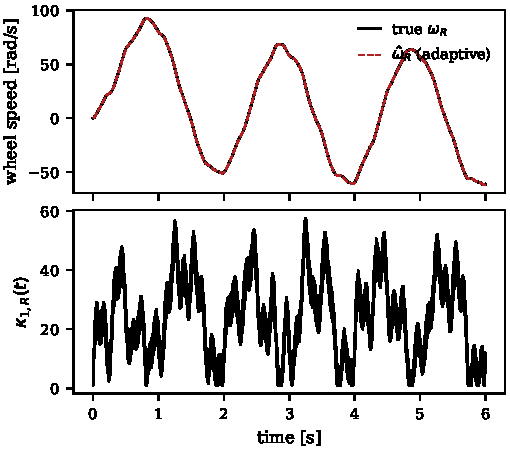
\includegraphics[width=0.9\linewidth]{fig_paper_tracking.pdf}
\caption{Right-wheel speed tracking on the nominal plant (top) and the corresponding adaptive gain $\kappa_{1,R}(t)$ (bottom). The gain settles in the range $10$--$60$ without the plant's inertial parameters, or a bound on wheel acceleration, ever being supplied to the observer.}
\label{fig:tracking}
\end{figure}

Fig.~\ref{fig:tracking} illustrates the closed-loop behavior obtained on the nominal plant. The observer tracks the true wheel velocity closely, and the adaptive gain varies with the excitation rather than remaining at a single, conservatively chosen value fixed in advance.

\subsection{Generalization across unknown plants}
\label{sec:genexp}
Sixty plants were generated by sampling $m\sim\mathcal{U}(1,6)$\,kg, $I_z\sim\mathcal{U}(0.01,0.08)$\,kg$\cdot$m$^2$, and $J_w\sim\mathcal{U}(5{\cdot}10^{-5},2{\cdot}10^{-4})$\,kg$\cdot$m$^2$ independently and uniformly at random, and each was driven with the same multi-sine excitation and the same observer and adaptive-law constants specified above. Table~\ref{tab:gen} summarizes the resulting observer and identification accuracy over the 60 trials; a bootstrap analysis (95\% confidence interval on the mean observer error of $[0.272,0.323]\%$, $N=5000$ resamples) confirms that this estimate is stable. Because $\beta$ changes sign over the sampled range, its percentage error is not meaningful for a subset of trials; Table~\ref{tab:gen} therefore reports its absolute error normalized by $\alpha_{\text{true}}$, which remains bounded away from zero throughout.

\begin{table}[h]
\centering
\caption{Accuracy over 60 random, unseen plants (no retuning)}
\label{tab:gen}
\begin{tabular}{lccc}
\hline
Metric & Mean & Std & Max$|\cdot|$\\
\hline
Observer RMS error & 0.30\% & 0.10\% & 0.46\%\\
$\alpha$ error & $-0.54\%$ & 0.26\% & 1.12\%\\
$\beta$ error (normalized)$^*$ & 0.46\% & 0.28\% & 1.10\%\\
$b$ error & $-1.76\%$ & 0.29\% & 2.25\%\\
\hline
\end{tabular}
\\ \raggedright \footnotesize $^*$absolute $\beta$ error divided by $\alpha_{\text{true}}$; see text.
\end{table}

\begin{table}[t]
\centering
\caption{Trajectory comparison (nominal plant, $\sigma_i=5$mA, 6 Monte Carlo trials per row; bold: best value per column)}
\label{tab:traj}
\scriptsize
\setlength{\tabcolsep}{2.8pt}
\begin{tabular}{lccccc}
\hline
Trajectory & $\alpha$ err. & $\beta$ err. & $b$ err. & Obs. RMS & $\sigma_{\min}$ \\
\hline
Common-mode & $-64.5\%$ & $-222\%$ & $-33.5\%$ & $1.76\%$ & $1.0{\times}10^3$\rlap{$^\dagger$} \\
Min. differential & $-1.54\%$ & $-5.25\%$ & $-52.9\%$ & $2.81\%$ & $2.7{\times}10^4$ \\
Multi-sine & $\mathbf{-0.36\%}$ & $\mathbf{-0.81\%}$ & $-35.5\%$ & $\mathbf{1.73\%}$ & $1.2{\times}10^5$ \\
PRBS & $-0.51\%$ & $-1.45\%$ & $\mathbf{-25.7\%}$ & $5.57\%$ & $2.4{\times}10^5$ \\
Chirp & $-5.97\%$ & $+2.29\%$ & $-55.5\%$ & $11.3\%$ & $7.8{\times}10^4$ \\
Figure-eight & $\mathbf{-0.36\%}$ & $-1.35\%$ & $-39.6\%$ & $2.00\%$ & $\mathbf{4.7{\times}10^5}$ \\
\hline
\end{tabular}
\\ \raggedright \footnotesize $^\dagger$equal to the RLS regularization floor $1/\delta$: no information is gained in this direction, the numerical signature of exact rank deficiency. Chirp spans $0.2$--$8$\,Hz.
\end{table}

\subsection{Trajectory design}
\label{sec:trajexp}
Six candidate excitation trajectories were compared on the nominal plant with $\sigma_i=5$\,mA (Table~\ref{tab:traj}): a common-mode-only input, serving as a negative control; a sine pair with minimal differential content; a multi-sine baseline; a pseudo-random binary sequence (PRBS); a linear chirp spanning $0.2$--$8$\,Hz; and a physically executable alternating drive-and-turn (``figure-eight'') maneuver. The quantity $\sigma_{\min}$ denotes the smallest singular value of the accumulated regressor $\Phi^\top\Phi$. The trajectories are not normalized to equal power, so $\sigma_{\min}$ reflects both the shape and the amplitude of the excitation, whereas the condition number $\sigma_{\max}/\sigma_{\min}$ is scale-invariant.

\begin{figure}[t]
\centering
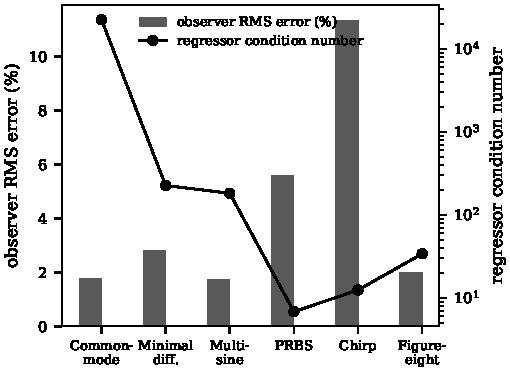
\includegraphics[width=0.9\linewidth]{fig_paper_traj.pdf}
\caption{Observer RMS error (bars, left axis) and regressor condition number (line, right axis, log scale) for each trajectory. PRBS and the chirp have lower regressor condition numbers than the multi-sine baseline yet produce larger observer errors; the common-mode-only input conditions poorly but is tracked without difficulty. Conditioning and realized accuracy are governed by different mechanisms.}
\label{fig:traj}
\end{figure}

Regressor conditioning and realized identification accuracy are found to decouple (Fig.~\ref{fig:traj}): PRBS and the chirp have condition numbers (6.8 and 12.4) far below that of the multi-sine baseline (182), yet the chirp yields the worst realized accuracy among the non-degenerate trajectories, and PRBS triples the observer's RMS error. This is attributed to the abrupt switching of PRBS and the fast frequency sweep of the chirp, both of which place greater demands on the adaptive-gain observer's tracking than smooth excitation; the resulting observer-level error propagates into the regression irrespective of its linear conditioning. The figure-eight maneuver attains the largest $\sigma_{\min}$ of all trajectories tested, although its condition number (34) exceeds that of PRBS and the chirp. Its $\alpha$ error equals that of the multi-sine baseline, and its $\beta$ error is about $0.5$ percentage points larger ($-1.35\%$ against $-0.81\%$). Unlike a multi-sine voltage command, it is directly executable by the robot in the field, and it is accordingly recommended as the excitation trajectory of choice.

\section{Discussion}
\label{sec:discussion}
\emph{Noise sensitivity of $b$.} Under current-sensor noise, the estimate $\hat\omega_k$ develops a bias that grows with $\sigma_i$, averaged over trials and measured directly as $+0.002$ to $-0.70$\,rad/s as $\sigma_i$ increases from $0$ to $20$\,mA, roughly an order of magnitude larger than that of a constant-gain observer subject to the same noise ($-0.05$\,rad/s at $20$\,mA). This bias arises from a rectification effect: the injection term $\sqrt{|e_k|}\,\mathrm{sign}(e_k)$ is odd but nonlinear, and its combination with the switching term $\mathrm{sign}(e_k)$ in $\dot z_k$ prevents symmetric current noise from averaging to zero drift, as it would through a linear observer. Because $b$ multiplies the filtered, DC-preserving quantity $\hat\omega_{k,f}$ directly in $\phi_k$ (Section~\ref{sec:rls}), whereas $\alpha$ and $\beta$ multiply the filtered-difference, DC-rejecting term $p(\hat\omega_k-\hat\omega_{k,f})$, this bias propagates into $b$ almost undiminished while leaving $\alpha$ and $\beta$ comparatively unaffected. This is confirmed on the nominal plant at $\sigma_i=20$\,mA, with $n=30$ trials per design: a constant-gain observer using the true, otherwise unavailable bound $\Delta_k$ achieves statistically significantly higher accuracy for all three parameters ($t=-3.0,-4.0,-730$ for $\alpha,\beta,b$, respectively; Welch test), an effect dominated by $b$. At $10$\,mA and below, with $n=12$ trials per design and noise level, this ordering is reversed for $\alpha$ and $\beta$, with $t$ between $6.7$ and $10.4$ favoring the adaptive design. This trade-off should be regarded as an open problem in applications where accurate estimation of $b$ under substantial sensing noise is required.

\emph{Operating range.} Identification accuracy also degrades at low wheel speed, through a mechanism independent of the one described above: restricting the platform to a narrow speed range trades a fixed sensor-noise floor against a diminishing signal amplitude. Over six excitation amplitudes at $\sigma_i=5$\,mA (four trials each), the observer RMS error and the error in $b$ both fall by a factor of about four between $\mathrm{RMS}\,\omega\approx4$\,rad/s and $\mathrm{RMS}\,\omega\approx22$\,rad/s, while the errors in $\alpha$ and $\beta$ fall by factors of about $3$ and $1.7$. Identification trials should therefore employ a sufficiently brisk excitation amplitude rather than an idled one.

\section{Conclusion}
\label{sec:conclusion}
A fixed-gain super-twisting observer for sensorless differential-drive identification requires a numerical bound on wheel acceleration derived from the very inertial parameters the identification pipeline is intended to recover, a circularity resolved here through a qualitative boundedness assumption and a boundary-layer adaptive gain law, supported by a self-contained finite-time gain-crossing guarantee (Proposition~\ref{prop:crossing}) and standard adaptive-gain super-twisting convergence (Theorem~\ref{thm:convergence}). The resulting design generalizes without retuning across a sixfold variation in chassis mass and an eightfold variation in yaw inertia (Table~\ref{tab:gen}). A physically executable figure-eight maneuver is shown to achieve accuracy comparable to that of the best trajectory considered, while trajectories with markedly lower regressor condition numbers yield worse accuracy, revealing a decoupling between conditioning and realized accuracy that a purely structural, rank-based criterion fails to capture (Table~\ref{tab:traj}). The principal open problem identified is a mechanistically explained sensitivity of the viscous-damping estimate to sensing noise (Section~\ref{sec:discussion}), which is left for future work.

\section*{Conflict of Interest}
The author declares no conflict of interest.

\section*{Acknowledgment}
Portions of the derivations, simulation code, and manuscript text in this letter were prepared with the assistance of Claude (Anthropic).

\begin{thebibliography}{1}
\bibitem{Levant1998} A. Levant, ``Robust exact differentiation via sliding mode technique,'' \emph{Automatica}, vol. 34, no. 3, pp. 379--384, 1998.
\bibitem{Moreno2012} J. A. Moreno and M. Osorio, ``Strict Lyapunov functions for the super-twisting algorithm,'' \emph{IEEE Trans. Autom. Control}, vol. 57, no. 4, pp. 1035--1040, 2012.
\bibitem{Plestan2010} F. Plestan, Y. Shtessel, V. Br\'{e}geault, and A. Poznyak, ``New methodologies for adaptive sliding mode control,'' \emph{Int. J. Control}, vol. 83, no. 9, pp. 1907--1919, 2010.
\bibitem{Shtessel2012} Y. Shtessel, M. Taleb, and F. Plestan, ``A novel adaptive-gain supertwisting sliding mode controller: Methodology and application,'' \emph{Automatica}, vol. 48, no. 5, pp. 759--769, 2012.
\bibitem{Bahrami2020} M. Bahrami, M. Naraghi, and M. Zareinejad, ``Adaptive super-twisting observer for fault reconstruction in electro-hydraulic systems,'' \emph{arXiv:2002.03411}, 2020.
\end{thebibliography}

\end{document}
